\section{数据测量}


本节介绍借助AI技术对单摆运动进行精确测量,获取用于计算重力加速度和阻尼系数的实验数据的实验步骤。

\subsection{实验装置准备}

将单摆装置放置在平稳桌面上,确保支架稳固,摆动时不会晃动;周围环境稳定,没有明显的振动和气流干扰小球的自然摆动。

\subsection{实验视频采集}

\begin{enumerate}[leftmargin=*]
    \item 相机设置与固定:
    \begin{itemize}
        \item 使用智能手机或数码相机,设置分辨率为1080p,帧率为60 FPS;
        \item 使用三脚架固定相机位置,确保镜头与单摆摆动平面严格平行;
        \item 调整相机距离,使单摆装置位于画面中央,且整个摆动过程都在视野范围内;
    \end{itemize}
    
    \item 初始条件设置:
    \begin{itemize}
        \item 使用精密刻度尺测量摆长$l$(从支点到摆球质心的距离),精确到毫米级,记录数值;
        \item 将摆球拉至特定初始角度$\theta_0$;
        \item 使用角度测量工具(如量角器)或底座刻度盘记录精确的初始角度值;
    \end{itemize}
    
    \item 视频拍摄执行:
    \begin{itemize}
        \item 轻柔释放摆球,避免施加额外力量,待摆球稳定摆动后开始拍摄;
        \item 拍摄时长:
        \begin{itemize}
            \item 重力加速度测量:保持拍摄至少5-10个完整周期(约10-20 s),提高统计精度;
            \item 阻尼系数测量:拍摄15-20个完整周期(约20-30 s),以充分捕捉振幅衰减过程;
        \end{itemize}
        \item 整个拍摄过程中保持环境安静,避免外部振动和气流干扰;
    \end{itemize}
    
    \item 多组数据采集:
    \begin{itemize}
        \item 重力加速度测量:重复测量摆长$l$,重复上述过程获取5组独立的实验视频,减小偶然误差;
        \item 阻尼系数测量:将摆长设置为0.8 m,重复上述过程获取5组独立的实验视频。
    \end{itemize}
\end{enumerate}
\begin{figure}[H]
    \centering
    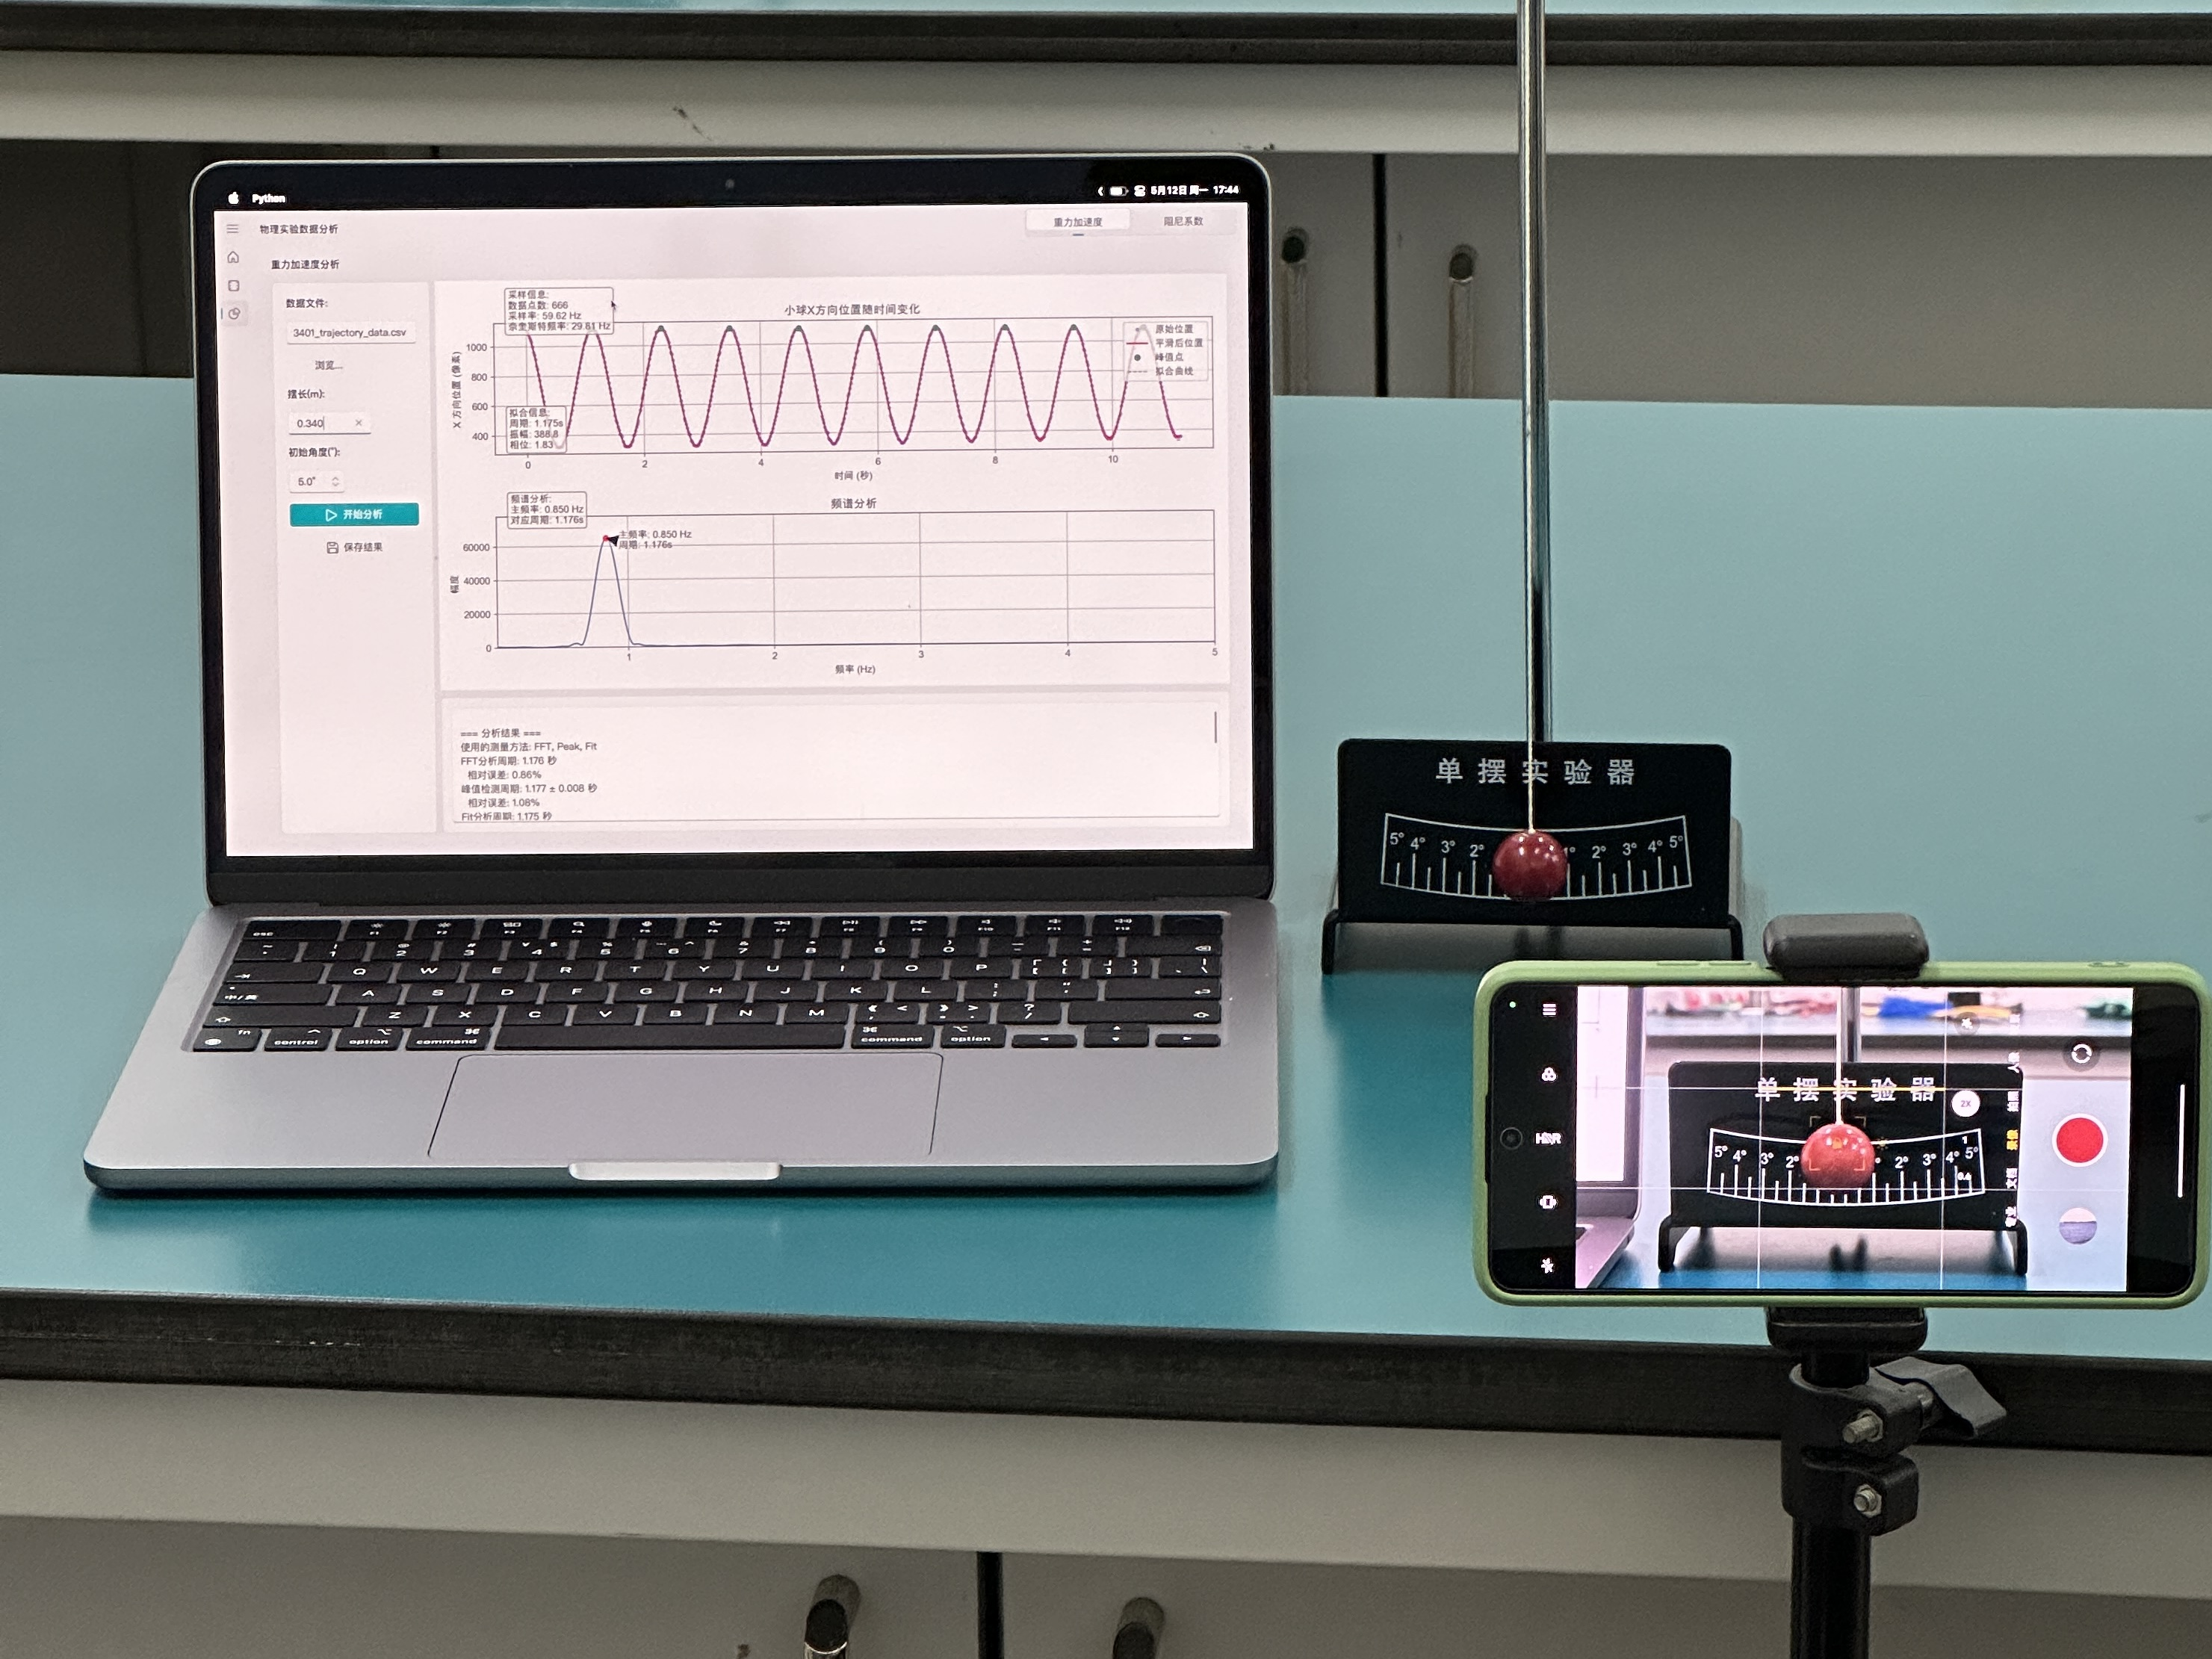
\includegraphics[width=0.6\textwidth]{figures/实验画面.JPG}
    \caption{实验数据采集过程}
    \label{fig:experiment_process}
\end{figure}

\subsection{实验数据处理与记录}

\begin{enumerate}[leftmargin=*]
    \item 软件初始化:启动实验分析软件,进入"视频处理"模块;
    
    \item 参数配置:
    \begin{itemize}
        \item 导入实验视频文件(支持MP4、AVI等主流格式);
        \item 载入训练完成的YOLO模型权重文件(默认为best.pt);
        \item 设置置信度阈值(默认为0.5,若检测效果不佳,可适当调低);
    \end{itemize}
    
    \item 数据提取执行:设置完参数后,点击"开始处理"按钮,启动AI识别模型,
    \begin{itemize}
        \item 观察实时预览窗口中摆球的检测框,确认跟踪稳定;
        \item 系统自动从每一帧提取摆球中心坐标,生成时间-位置原始数据集,保存为CSV格式文件;
        \item 处理完成后,点击结果文件夹按钮,可查看结果视频、轨迹图、位置-时间数据集;
    \end{itemize}

    \item 数据记录:
    \begin{itemize}
        \item 得到摆球位置-时间数据集文件后,进入"数据分析"模块;
        \item 选择分析模式:
        \begin{itemize}
            \item 重力加速度测量:选择"重力加速度测量"模式,输入摆长$l$与初始角度$\theta_0$,系统自动计算周期$T$与重力加速度$g$;
            \item 阻尼系数测量:选择"阻尼振动分析"模式,系统自动拟合振幅衰减曲线,计算阻尼系数$\beta$;
        \end{itemize}
        \item 将相关数据记录于实验记录表中。
    \end{itemize}   
\end{enumerate} 

\begin{figure}[H]
    \centering
    \subfigure[重力加速度测量结果]{
        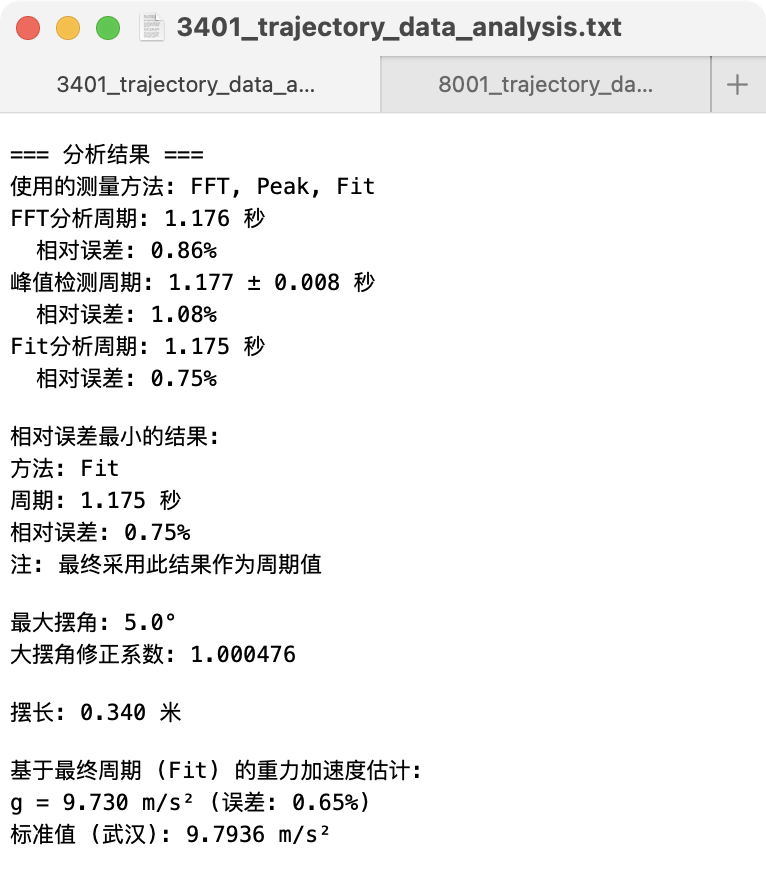
\includegraphics[width=0.4\textwidth]{figures/测量结果1.png}
        \label{fig:measurement_result1}
    }
    \subfigure[阻尼系数测量结果]{
        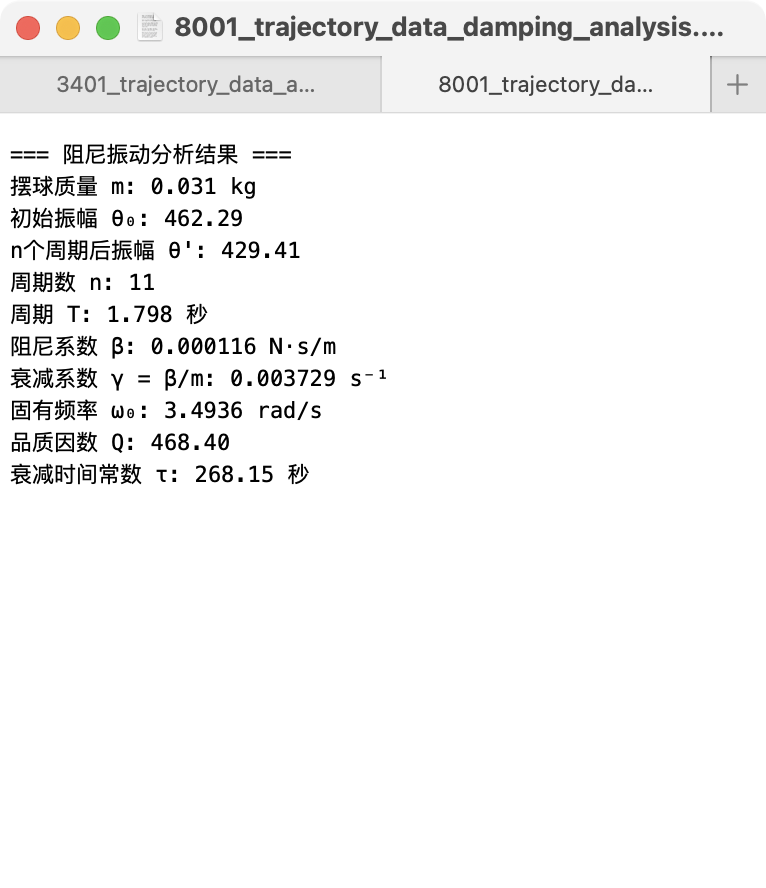
\includegraphics[width=0.4\textwidth]{figures/测量结果2.png}
        \label{fig:measurement_result2}
    }
    \caption{实验测量结果示例}
    \label{fig:measurement_results}
\end{figure}

